\providecommand{\main}{../..}
\documentclass[\main/thesis.tex]{subfiles}

\begin{document}

\section{General Observations}
Now we study simulations where carcinogens are present and cause mutations and, ultimately, cancer. Figure \ref{fig:GeneralObservations_importantTimeSteps} illustrates the development of a cancer field and tumours within it, where nicotine and ethanol are simulated using carcinogen spatial distribution 2 equation \eqref{eq:CarcinFunc2}. The various time-steps show (a) the initial seed, (b) the cancer field at its early development, (c) the cancer field further developing prior to cancer, in (d)-(f) the multiple stages of cancer development.  The colour map for the cell classes is as provided in Table \ref{table:CAStates}. The cancer field is initially minimal and undeveloped, but over time it evolves and matures, eventually forming tumours. These tumours grow and outpace the growth rate of the cancer field, as observed from the time-steps in Figures \ref{fig:GeneralObservations_lateTumour} and \ref{fig:GeneralObservations_final}. Note that in the time-step within Figure \ref{fig:GeneralObservations_lateTumour} the tumour masses near the edge of the field begin to explore beyond the field.
\begin{figure}[H]
    \centering
    \begin{subfigure}[t]{.45\textwidth}
      \centering
      
\includegraphics[width=\textwidth]{images/2_GeneralObservations/Fig5/1_init.jpeg}
      \caption{Initial seed}
      \label{fig:GeneralObservations_initSeed}
    \end{subfigure}
    \begin{subfigure}[t]{.45\textwidth}
      \centering
      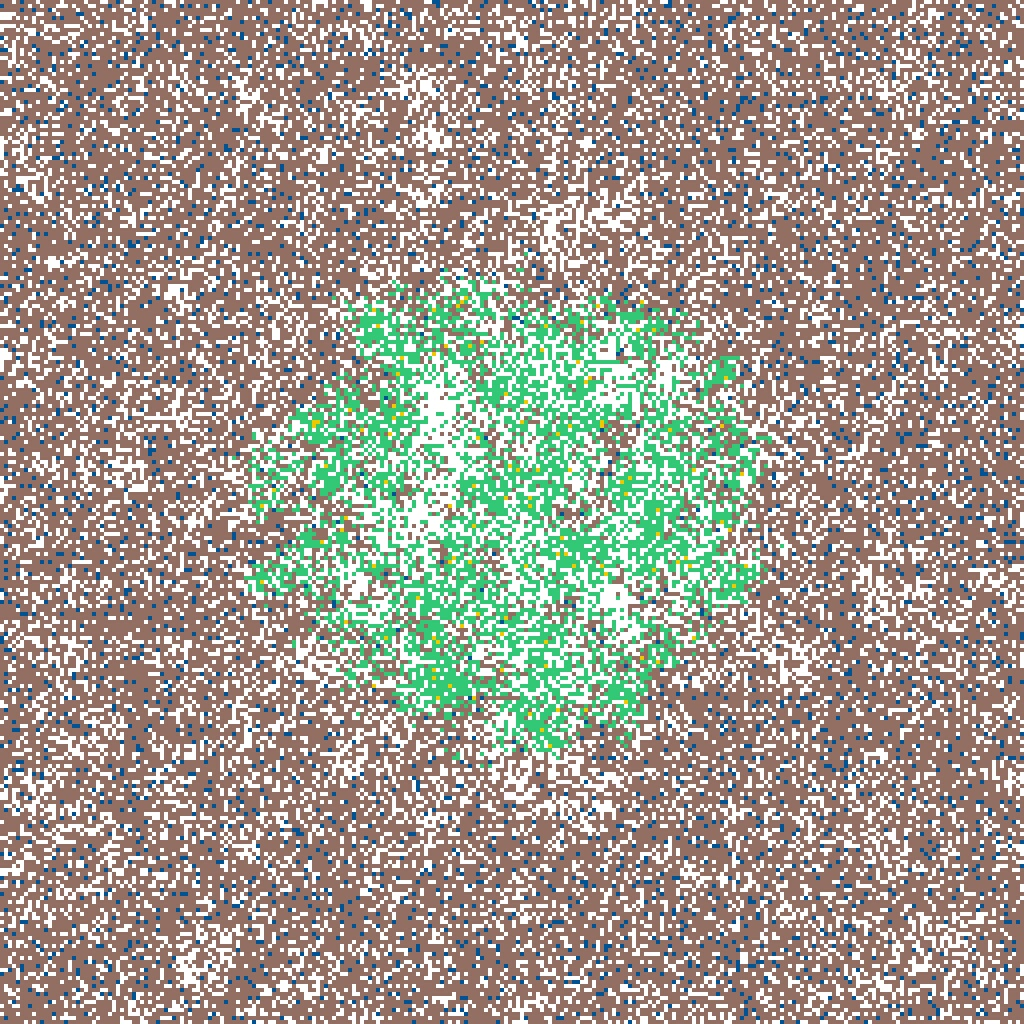
\includegraphics[width=\textwidth]{images/2_GeneralObservations/Fig5/2_early_field_1000.jpeg}
      \caption{Early field development, time-step 1000}
      \label{fig:GeneralObservations_earlyField}
    \end{subfigure}
    \begin{subfigure}[t]{.45\textwidth}
      \centering
      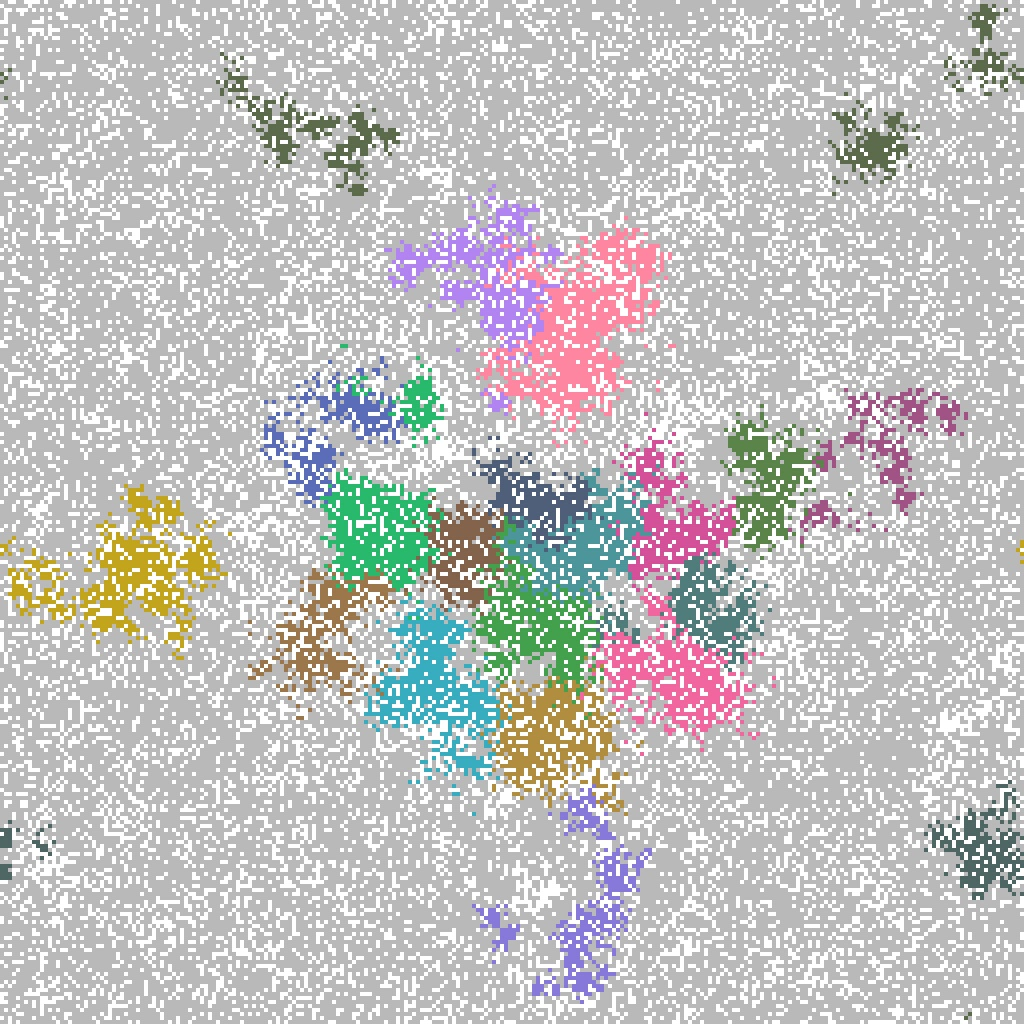
\includegraphics[width=\textwidth]{images/2_GeneralObservations/Fig5/3_late_field_1400.jpeg}
      \caption{Late field development, time-step 1400}
      \label{fig:GeneralObservations_lateField}
    \end{subfigure}
    \begin{subfigure}[t]{.45\textwidth}
      \centering
      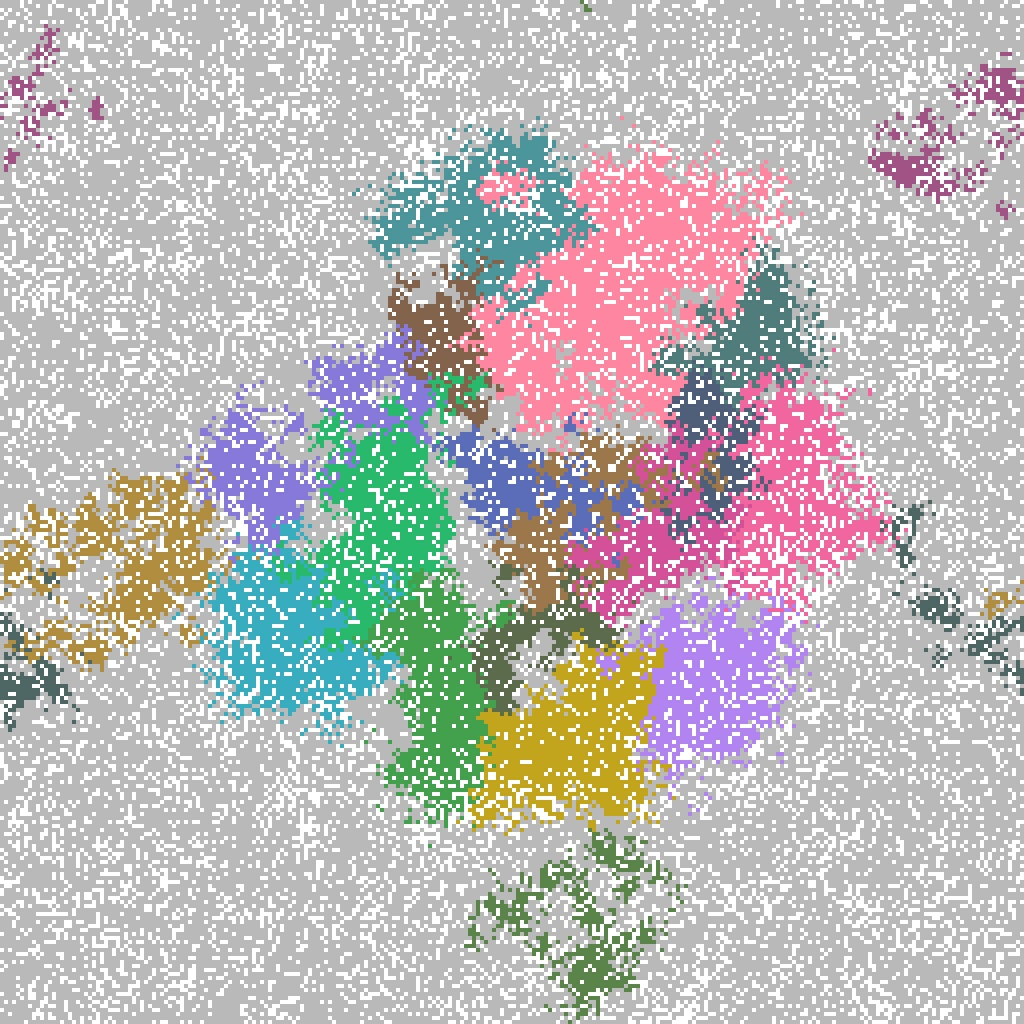
\includegraphics[width=\textwidth]{images/2_GeneralObservations/Fig5/4_early_tumour_1975.jpeg}
      \caption{Early cancer development, time-step 1975}
      \label{fig:GeneralObservations_earlyTumour}
    \end{subfigure}
    \begin{subfigure}[t]{.45\textwidth}
      \centering
      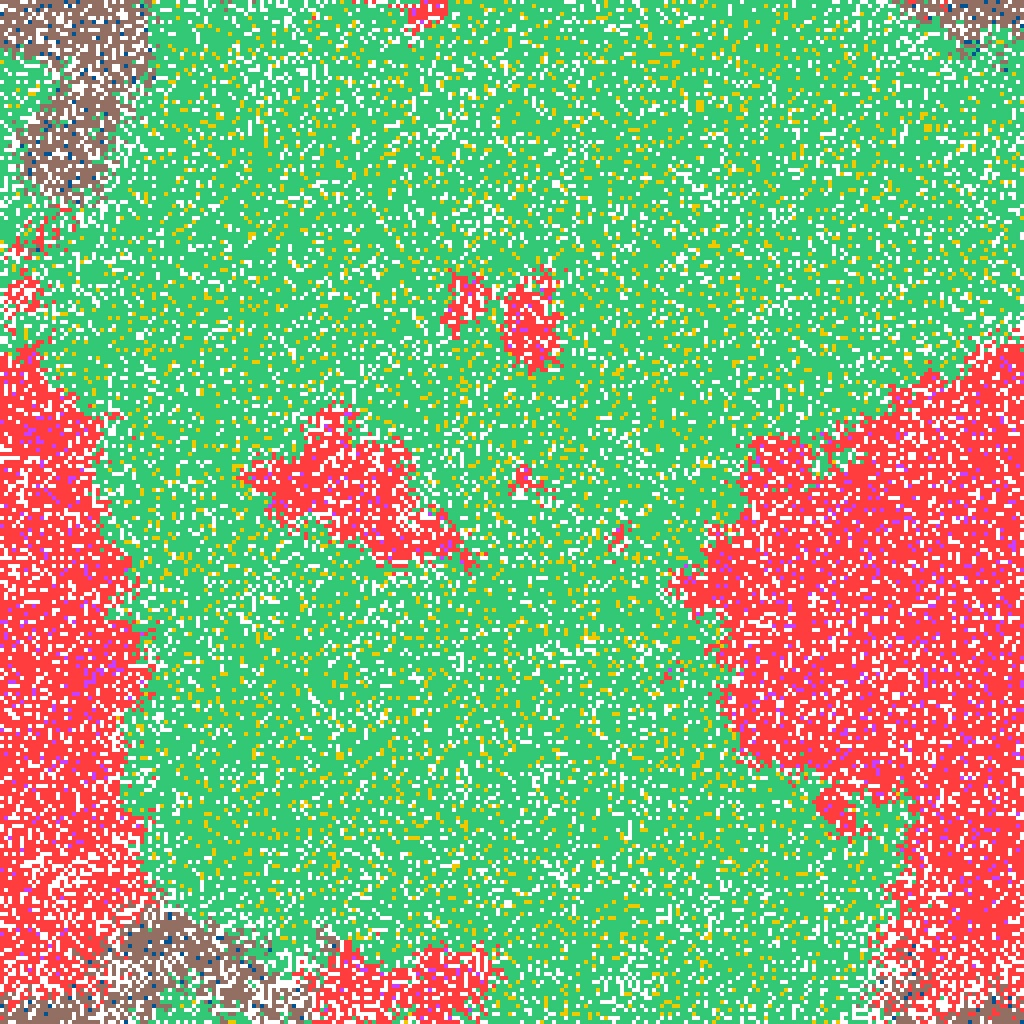
\includegraphics[width=\textwidth]{images/2_GeneralObservations/Fig5/5_late_tumour_3947.jpeg}
      \caption{Late cancer development, time-step 3947}
      \label{fig:GeneralObservations_lateTumour}
    \end{subfigure}
    \begin{subfigure}[t]{.45\textwidth}
      \centering
      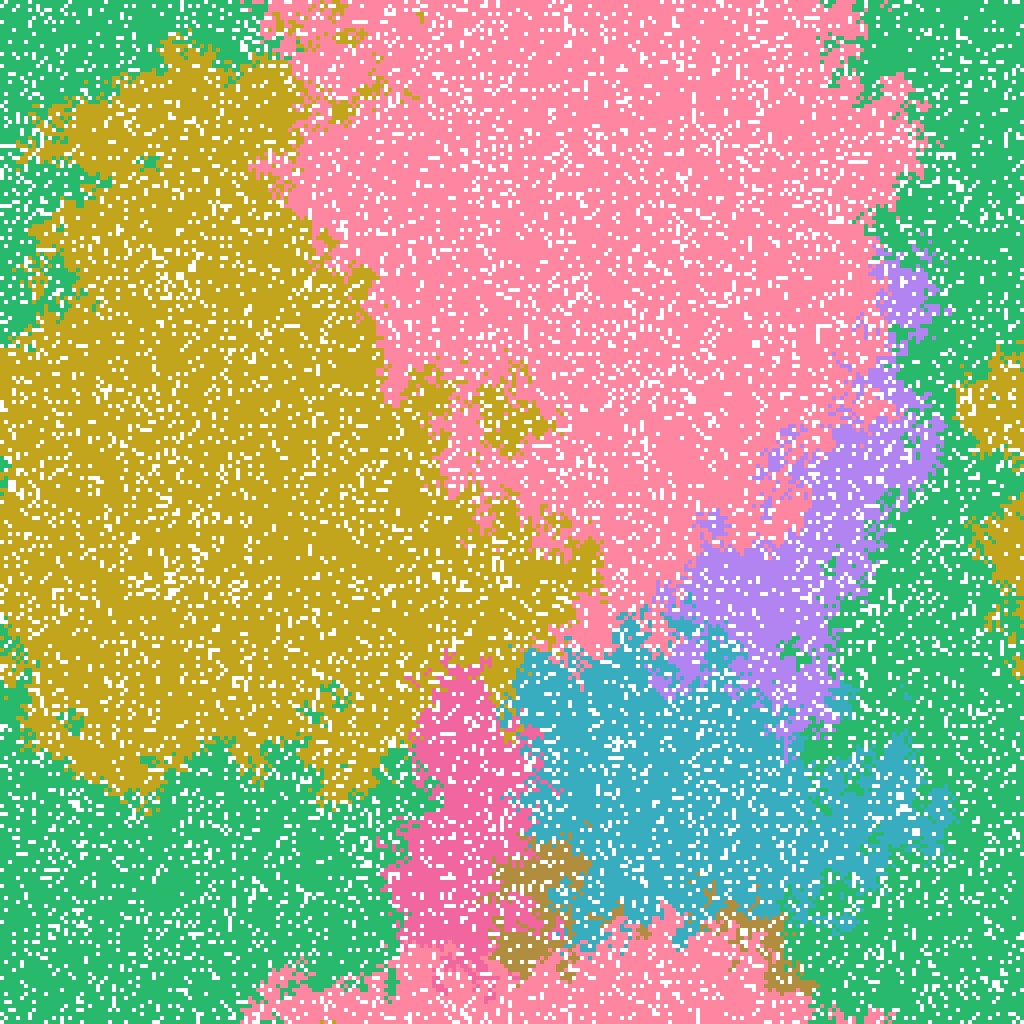
\includegraphics[width=\textwidth]{images/2_GeneralObservations/Fig5/6_final.jpeg}
      \caption{Final time-step, time-step 8766}
      \label{fig:GeneralObservations_final}
    \end{subfigure}
    \caption{This figure includes time-steps illustrating the development of a cancer field and cancer cells using the colour map for the cell classes as provided in Table \ref{table:CAStates}. These show (a) the initial seed, (b) the cancer field at its early development, (c) the cancer field further developing but prior to cancer, (d) the first stages of cancer development, (e) further cancer growth, and (f) the final time-step. Parameters are as follows: grid size 256x256, carcinogen spatial distribution 2, both carcinogens activated.}
    \label{fig:GeneralObservations_importantTimeSteps}
\end{figure}

\subsection{Field Development}
Regardless of changes to parameters, other than carcinogens activated, we observe that the field begins to form where the carcinogen is most concentrated; this can be verified with Figure \ref{fig:GeneralObservations_earlyField} (early field development) and \ref{fig:CarcinFunc_Func2Distribution} (visual representation of the carcinogen spatial distributions used in 4.4b). Initially, the field is made up of only mutated normal tissue cells (green cells) and mutated normal stem cells (yellow cells), as shown in Figure \ref{fig:GeneralObservations_earlyField}. Typically, the first mutated cell is a MNTC due to there being a higher number of NTC compared to NSC. The field grows outwards as it takes over normal tissue. 
 
 In Figure \ref{fig:GeneralObservations_FieldGrowth} we show the time evolution of the fraction of mutated cells. We defined the cancer field as the areas of the domain that contain cells from the mutated cell classes thus, the figure shows the cancer field growth over time. 
 \begin{figure}[H]
    \centering
    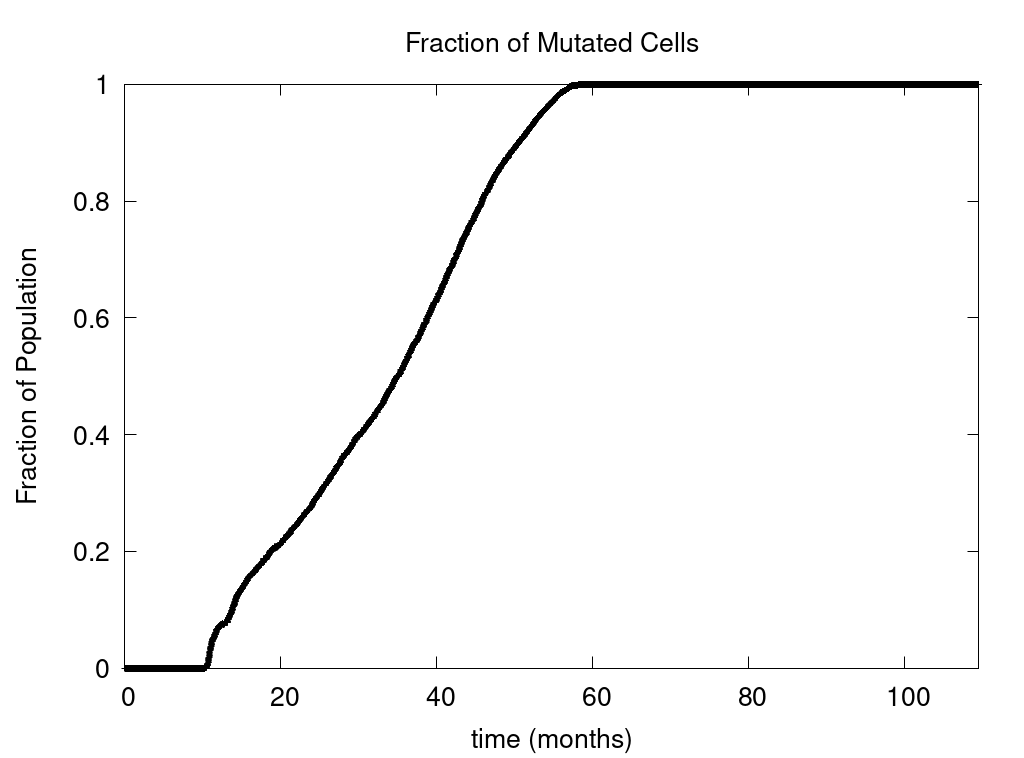
\includegraphics[scale=0.25]{images/2_GeneralObservations/Fig4/numMutated.png}
    \caption{This figure shows the time course of the fraction of mutated cells, thus illustrating the cancer field growth over time. Parameters are as follows: grid size 256x256, carcinogen spatial distribution 2, both carcinogens activated.}
    \label{fig:GeneralObservations_FieldGrowth}
\end{figure}
 The point at which the curve begins its rapid linear growth is that time for which the first mutated cell appears, this line flattens at the time in which the carrying capacity of the domain is achieved. Field growth rate initially starts off moderately, briefly slows, finally becoming aggressive. The period of slow growth is related to empty cells being unusually abundant because the mutated cells are not yet aggressive enough to overtake the empty cells, nor is the stem cell to normal tissue cell ratio stabilized at this point. Further evidenced by Figure \ref{fig:GeneralObservations_earlyField} which shows patches of empty cells (white) within the field and very few stem cells (yellow) at this point.
Figure \ref{fig:GeneralObservations_FieldGrowth} illustrates that once the field has developed and grown large enough, the odds of a NSC or MNSC becoming a CSC increases. Soon after the emergence of the first CSC, TCs begin to form. 
% Show this with figure
Note that the TCs will die off if the first TC's fitness is too low compared to neighbouring cells, or if the CSC that created the TCs dies off.
Once the tumour mass within the field itself starts to form, TCs and CSCs eventually take over the entire field, as shown in Figures \ref{fig:GeneralObservations_earlyTumour}-\ref{fig:GeneralObservations_final}. This phenomenon is a result of having limited space, and other mutated cells not being as aggressive and fit as the tumour cells. % Show with growth curves

\subsection{Tumour Growth Rate}
In Figure \ref{fig:GeneralObservations_TumourMassGrowthCurve} we show the time evolution of the fraction of CSC and TCs which together form the tumour mass. We observe that the tumour follows logistic growth which is due to domain spatial limitations.
\begin{figure}[H]
    \centering
    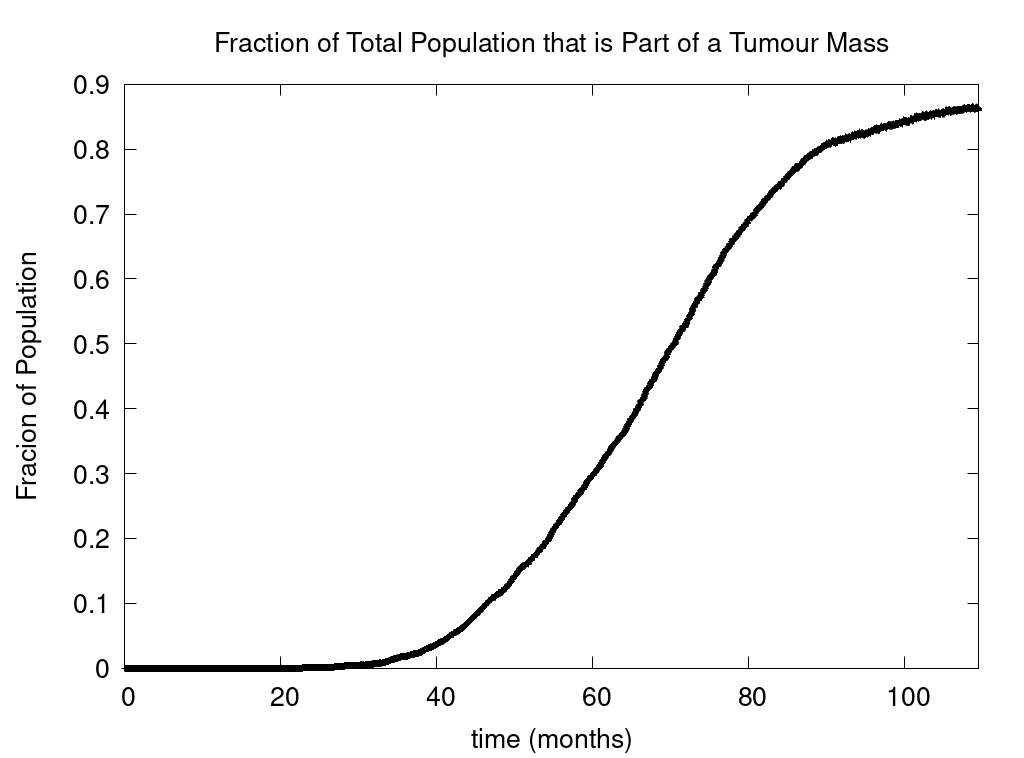
\includegraphics[scale=0.25]{images/2_GeneralObservations/Fig1/numCSCAndTC.png}
    \caption{This figure shows the time course of the fraction of CSC and TC, thus illustrating the tumour growth over time. Parameters are as follows: grid size of 256x256, carcinogen spatial distribution 2, both carcinogens activated.}
    \label{fig:GeneralObservations_TumourMassGrowthCurve}
\end{figure}
Growth is initially quite slow but rapidly increases as the cells become more aggressive from the accumulated mutations. The growth flattens, never quite achieving 100\% due to the aforementioned spatial limitations of the domain and the domain still also containing some CSCs and empty cells. Theoretically, with an infinite or growing domain the growth curves would be exponential. However, a fixed domain is more realistic biologically speaking due to the fact that the tissue  surrounding the tumour has limited space. Therefore, the growth of a tumour within a given tissue should follow logistic growth, which our model confirms. 

\subsection{Mutational Evolution}
Recall we use the term ``positive mutation" to portend that a mutation promotes cancer, (i.e., upregulation of an oncogene or downregulation of a tumour suppressor gene). 
In Figure \ref{fig:GeneralObservations_GeneEvo} we show various graphs that represent the mutational evolution of the genes over time. In (a) and (b) the average gene expression is illustrated for first the tumour suppressors and secondly the oncogenes. In (c) we show the time evolution of the fraction of genes that are positively mutated. 
In Figure \ref{fig:GeneralObservations_TumourSuppressors} all the tumour suppressor genes are downregulated, hence positively mutated. Other than RB, which decreases at a faster rate, the gene expressions of all the other tumour suppressor genes decrease at a similar rate. Figure \ref{fig:GeneralObservations_Oncogenes} displays that the oncogenes are upregulated, therefore positively mutated. The gene expressions of the oncogenes increase at a similar rate except CCDN1 and RAS, which increase at a faster rate. In Figures \ref{fig:GeneralObservations_TumourSuppressors} and \ref{fig:GeneralObservations_Oncogenes} we see that the gene expressions between the genes can vary significantly, principally with P21 and CCDN1. These two genes mutate because they are related to the most genes, and therefore have a higher weight in the MLP output weight matrix, $W_y$, in equation \eqref{param:Wy}.
\begin{figure}
    \centering
    \begin{subfigure}[t]{.65\textwidth}
      \centering
      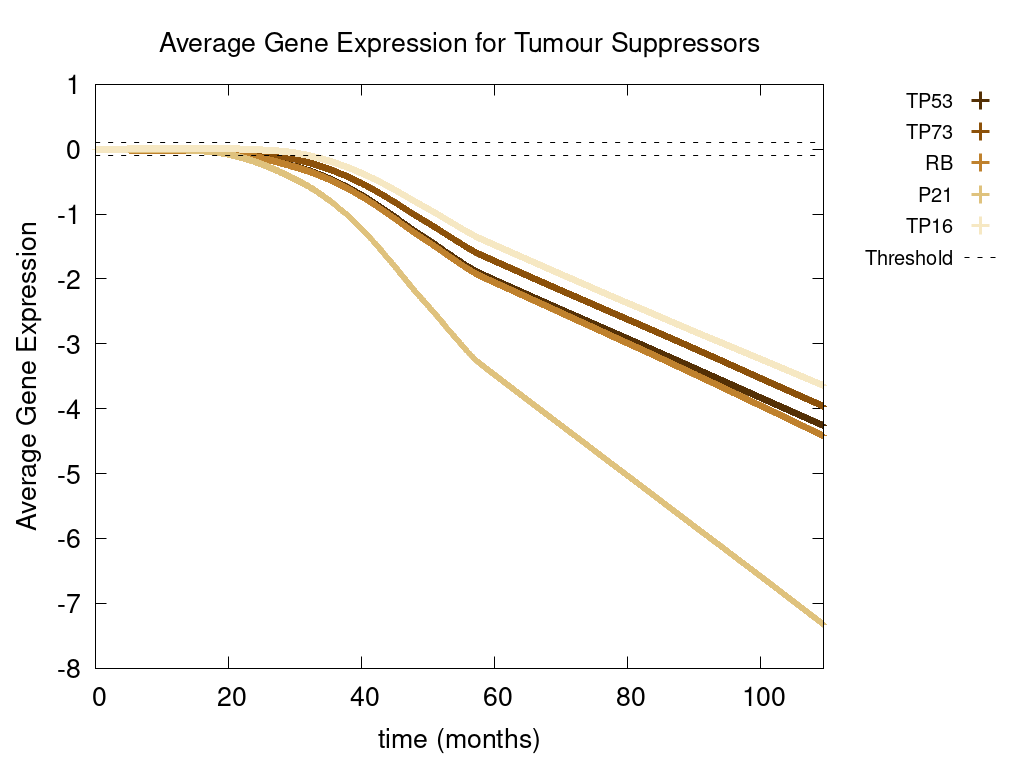
\includegraphics[width=\textwidth]{images/2_GeneralObservations/Fig2/geneExprAll_TumourSuppressors.png}
      \caption{Tumour suppressor gene expression over time}
      \label{fig:GeneralObservations_TumourSuppressors}
    \end{subfigure}
    \begin{subfigure}[t]{.65\textwidth}
      \centering
      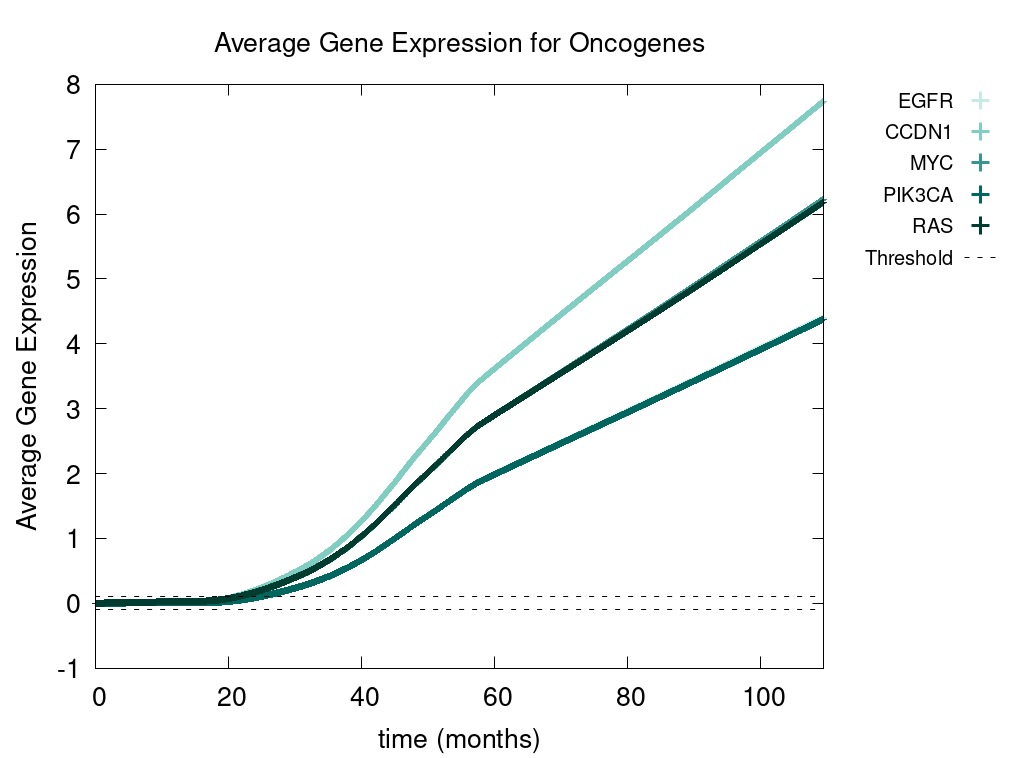
\includegraphics[width=\textwidth]{images/2_GeneralObservations/Fig2/geneExprAll_Oncogenes.png}
      \caption{Oncogene gene expression over time}
      \label{fig:GeneralObservations_Oncogenes}
    \end{subfigure}
    \begin{subfigure}[t]{.55\textwidth}
      \centering
      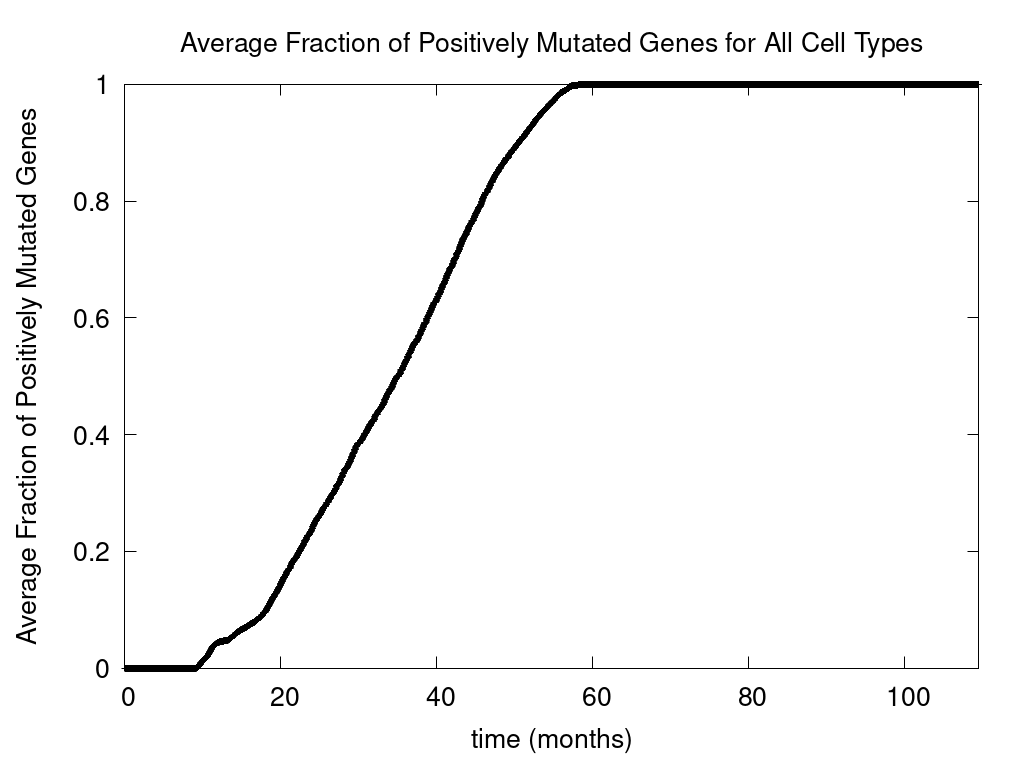
\includegraphics[width=\textwidth]{images/2_GeneralObservations/Fig2/numPosMut_all.png}
      \caption{Fraction of positively mutated genes over time}
      \label{fig:GeneralObservations_numPosMut}
    \end{subfigure}
    \caption{In this figure we show the mutational evolution of the genes. The time course of the average gene expression are shown for in (a) the tumour suppressor genes, in (b) the oncogenes. In (c) we show the time course of the fraction of genes that are positively mutated. Parameters were chosen as follows: grid size of 256x256, carcinogen spatial distribution 2 was used, both carcinogens were activated.}
    \label{fig:GeneralObservations_GeneEvo}
\end{figure}

Figure \ref{fig:GeneralObservations_numPosMut} shows a lag of time before the first positively mutated genes occur, this is due to the low mutational rate, and competition against the body trying to revert mutations. The initial spike in mutational rate at the onset of the first mutated cell is due to the relative size of the domain versus the mutated cells. Once multiple genes become positively mutated the progression accelerates, due to changes in the expression of other genes caused by genetic instability, as displayed in the period starting at about 20 to 25 months. Referring to Figures \ref{fig:GeneralObservations_TumourSuppressors} and \ref{fig:GeneralObservations_Oncogenes} we can observe that all the genes are positively mutated by about 25 months. Once TP53 is positively mutated, genes will become cancerous, as it correlates to cell cycle arrest and can make a cell apoptotic, due to genetic mutations.

\subsection{Phenotypic Evolution}
Next we consider the evolution of a phenotypic action, which includes proliferation, quiescence, apoptosis, and differentiation as functions of time. 
Figure \ref{fig:GeneralObservations_PhenoEvo} illustrates the phenotypic evolution of these actions as (a) the time evolution of the fraction of cells that underwent each phenotypic action and in (b) the time evolution of the average probability for each of these. Figure \ref{fig:GeneralObservations_chancePheno} demonstrates the probability of apoptosis occurring decreases as the cell population moves towards being cancerous. This occurs mathematically with time as the majority of the genes become positively mutated causing apoptosis to decrease as expected due to the genes modifying the probability of apoptosis. While the probability of apoptosis decreases, the chance of proliferation and differentiation increases, this again is caused by how the positively mutated genes influence the probability of proliferation and differentiation. Probability of differentiation increases at a slower rate than proliferation because fewer of the genes we consider influence differentiation. Finally, for the most part, the probability of quiescence remains stable - it goes slightly up and down, due to being balanced against the other phenotypic actions, and not many genes are influencing it, but otherwise it is at equilibrium. Figure \ref{fig:GeneralObservations_numPheno} shows us that apoptosis and proliferation change the most over time, in particular, as apoptosis decreases, we see that proliferation increases, due to less cells dying before they can become more cancerous. This figure reveals that quiescence (movement) initially increases when the field begins forming as the field contains an insufficient number of mutated stem cells to thrive, consequently there will be more empty cells.
\begin{figure}[H]
    \centering
    \begin{subfigure}[t]{.65\textwidth}
      \centering
      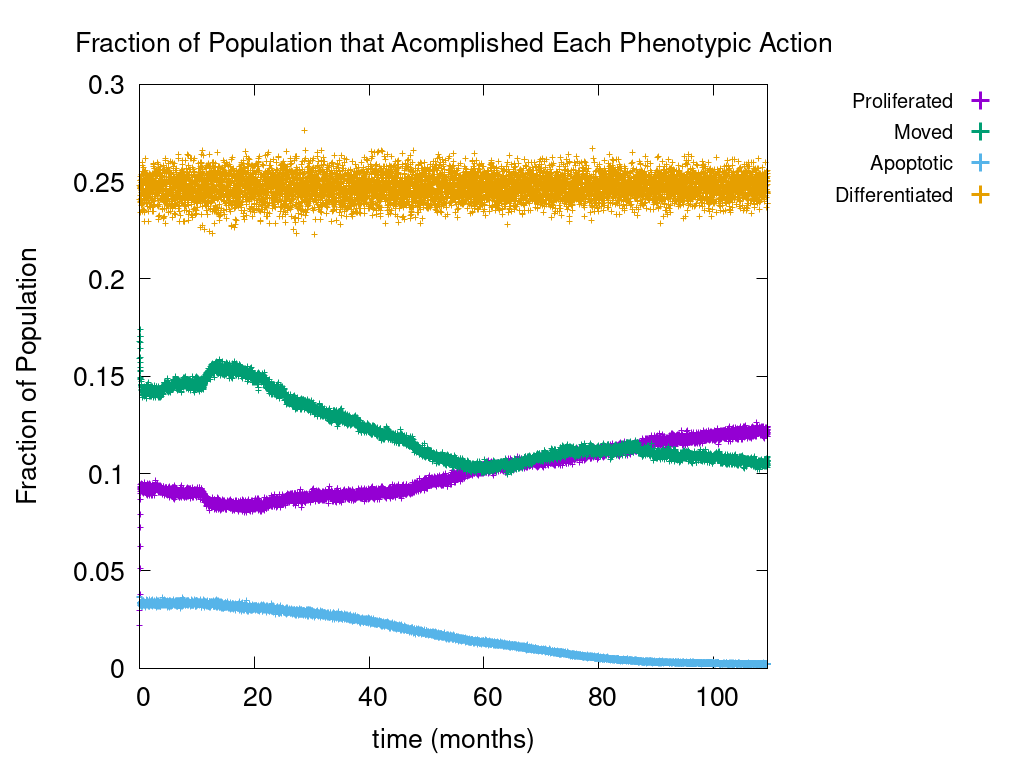
\includegraphics[width=\textwidth]{images/2_GeneralObservations/Fig3/numPheno_all.png}
      \caption{Fraction of cells undergoing each phenotypic action}
      \label{fig:GeneralObservations_numPheno}
    \end{subfigure}
    \begin{subfigure}[t]{.65\textwidth}
      \centering
      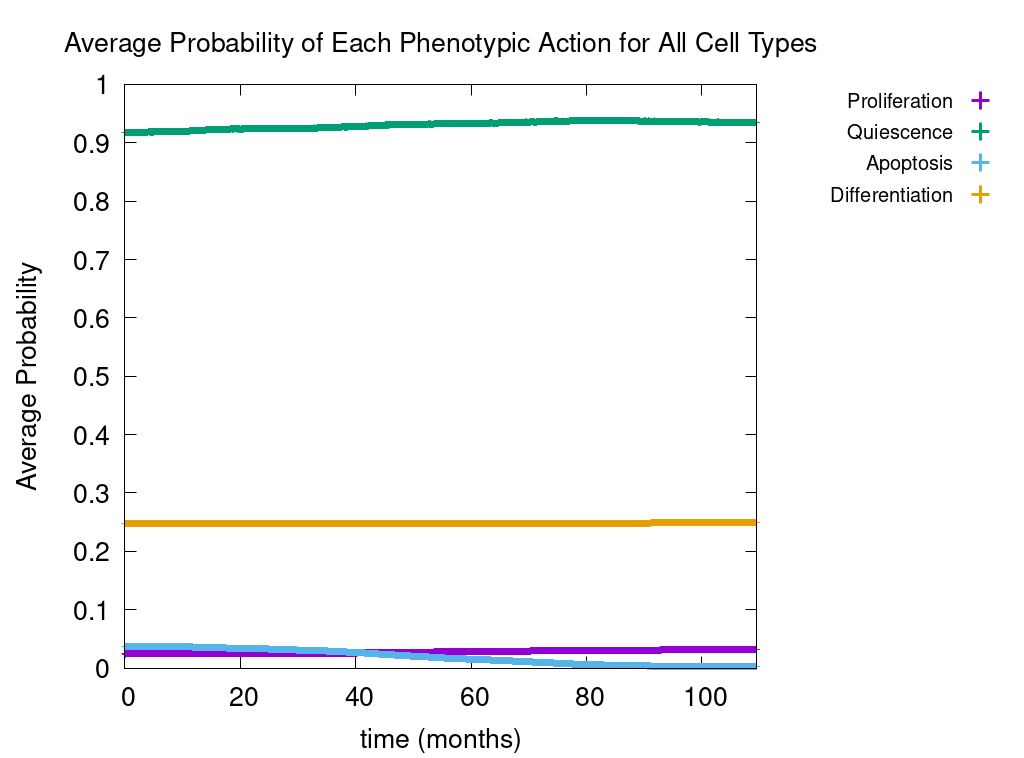
\includegraphics[width=\textwidth]{images/2_GeneralObservations/Fig3/chancePheno_all.png}
      \caption{Average probability for each phenotypic action over time}
      \label{fig:GeneralObservations_chancePheno}
    \end{subfigure}
    \caption{This figure illustrates the phenotypic evolution of proliferation, apoptosis, quiescence, and differentiation. In these we show (a) the time course of the fraction of cells that underwent each phenotypic action and (b) the time course of the average probability for each phenotypic action. Parameters are as follows: grid size 256x256, carcinogen spatial distribution 2, both carcinogens activated.}
    \label{fig:GeneralObservations_PhenoEvo}
\end{figure}
 

\end{document}